\documentclass{article}

% Language setting
% Replace `english' with e.g. `spanish' to change the document language
\usepackage[english]{babel}
\usepackage{listings}
\usepackage{xcolor}
\usepackage{graphicx} % Required for inserting images
\usepackage{amsmath}
\usepackage{esvect}
\usepackage{booktabs}
\usepackage{float}
\usepackage{enumerate}
\usepackage{hyperref}

\definecolor{codegreen}{rgb}{0,0.6,0}
\definecolor{codegray}{rgb}{0.5,0.5,0.5}
\definecolor{codepurple}{rgb}{0.58,0,0.82}
\definecolor{backcolour}{rgb}{0.95,0.95,0.92}

\lstset{language=Python, 
        basicstyle=\ttfamily\small,
        backgroundcolor=\color{backcolour},
        commentstyle=\color{codegreen},
        stringstyle=\color{red},
        basicstyle=\ttfamily\footnotesize,
        showstringspaces=false,
        keywords=[2]{pow},
        keywordstyle=[2]{\color{orange}},
}
% Set page size and margins
% Replace `letterpaper' with `a4paper' for UK/EU standard size
\usepackage[letterpaper,top=2cm,bottom=2cm,left=3cm,right=3cm,marginparwidth=1.75cm]{geometry}

% Useful packages
\usepackage{amsmath}
\usepackage{graphicx}
\usepackage[colorlinks=true, allcolors=blue]{hyperref}

\title{\textbf{Secure Multi-Party Computation
} \hspace{10cm} 
Assignment 2 - One-Time-Truth-Table for computing a function with 2 parties\textbf{}}
\author{Or Dinar \\
Liad Ackerman}
\date{25.01.2024}

\begin{document}
\maketitle

\section{OTTT for 2 Participants - Theory}

In this assignment we were given an equation, and our task is to use OTTT (One-Time-Truth-Table) protocol to securely compute the result.
\newline
\newline
Reminder:

$$
f_{a,4}(x)=\begin{cases}
			1 & \text{if $ax \geq 4$ }\\
                0 & \text{otherwise}
		  \end{cases} \hspace{1cm} for \hspace{.25cm}a\in \left\{0,1,2,3\right\}
$$
\begin{figure}[H]
    \centering
    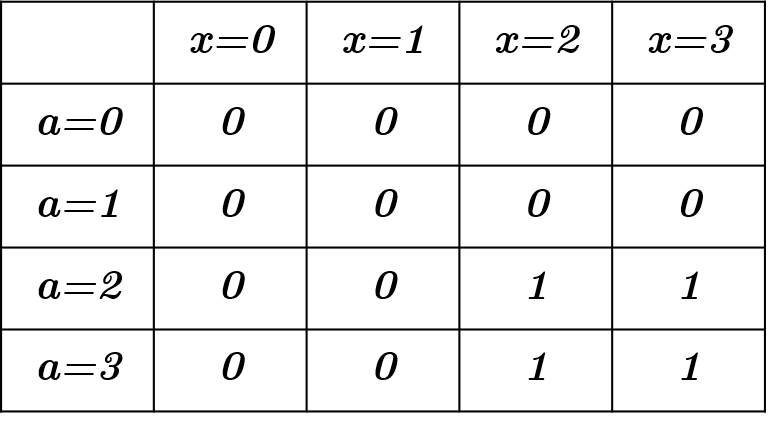
\includegraphics[width=0.5\linewidth]{Picture1.png}
    \caption{Truth-table for equation 2.}
    \label{fig:enter-label}
\end{figure}

\subsection{Dealer}
We learned in the lecture 3 that OTTT uses a trusted party in order to securely compute an output for a function. The dealer party gets the truth table $T$ for the function $f$, it draws a random $(r,c) \in \left\{0,1,...,2^n\right\}$, and it also creates a matrix $M_{B}$ 
 with random values from $\left\{0,1\right\}$ for each cell,which is of the same dimensions as $T$ (both are $2^n \times 2^n$). For our function $f$ the dimensions of $T$ and $M_B$ are $2^2 \times 2^2$.

Once the dealer gets all of the mentioned information, it alters $T$ by shifting the rows $r$ times, and shifting the columns $c$ times. After the altercation of $T$, Dealer computes a new matrix denoted as $M_A$, by performing $M_A = M_B \bigoplus T$ for the altered $T$. Dealer then sends $(r,M_A)$ to Alice (first party), and $(c,M_B)$ to Bob (second party).

\subsection{First Party (Alice)}
\subsubsection{Send}
Alice has $(r,M_A)$ and her input $x$, the computation she performs is:
$$
    u = x + r \hspace{.1cm} mod \hspace{.1cm} 2^2
$$
Then Alice sends $u$ to Bob.

\subsubsection{Recieve}
Alice receives $(v,Z_B)$ from Bob, which are two scalars. With the given data she computes $z$ (The output of the function $f$) like so:
$$
    z = M_A[u,v] \bigoplus Z_B
$$
\textbf{which is the final result for $f$.}

\subsection{Second Party (Bob)}
\subsubsection{Recieve}
Bob has his input $a$, $(c,M_B)$ from Dealer, and he recieves $u$ from Alice. With the given information Bob computes:
\newline
1.)
$$
    v = y + c \hspace{.1cm} mod \hspace{.1cm} 2^2
$$
2.)
$$
    Z_B = M_B[u,v]
$$

\subsubsection{Send}
Bob sends the values he computed $(v,Z_B)$ to Alice for further computation.

\section{OTTT for 2 Participants - Implementation}
The implementation of the OTTT protocol is in the script $HW2.py$ attached to the zip file submitted. The script itself is well documented but we will still explain it to some extent in this paper.
\newpage

\subsection{Dealer Class}
The implementation for Dealer class captures: getting the data for the Dealer party, getting a random $(r,c)$ and shifting rows and columns of $T$ accordingly, creating a matrix $M_B$ of randomized values from $\left\{0,1\right\}$, and calculating $M_A$.
\begin{lstlisting}
class Dealer:
    def __init__(self):
        # set truth table for equation 2, table is going to be a 4x4 numpy array 
        # rows = a's value, column = x's value
        self.table = pd.read_csv('truth_table.csv').to_numpy()
        
        # shifts[0] shifts for rows
        # shifts[1] shifts for columns
        shifts = np.array([np.random.choice(range(1,5)),np.random.choice(range(1,5))])
        
        #assigning shift values to the class' variables
        self.r = shifts[0]
        self.c = shifts[1]
        
        # shift table rows anc columns
        self.table = shiftRows(self.table,shifts[0])
        self.table = shiftCols(self.table,shifts[1])
        
        # randomized matrix the size of 4x4 (like the truth table for equation 2)
        # this matrix will be sent to Bob
        self.matrixB = [[np.random.choice([0, 1]) for _ in range(4)] for _ in range(4)]
        
        # compute matrixA for the dealer to send to Alice
        self.matrixA = np.bitwise_xor(self.table, self.matrixB)
        ...
\end{lstlisting}

The functions RandA and RandB return the values that Alice and Bob should get from the trusted Dealer.
\begin{lstlisting}
class Dealer:
    ...
    def RandA(self):
            # give Alice (r, Ma)
            return (self.r, self.matrixA)
    
    def RandB(self):
        # give Bob (c,Mb)
        return (self.c, self.matrixB)
\end{lstlisting}

\subsection{Alice Class}
The implementation for Alice class captures: getting the data from Dealer and performing the calculations mentioned on the previous section.
\begin{lstlisting}
class Alice:
    def __init__(self,input, dealerOut):
        self.input = input
        self.r = dealerOut[0]
        self.matrix = dealerOut[1]
        
    def Send(self):
        # Alice sends Bob u = x + r mod 4
        self.u = (self.input + self.r) % 4
        return self.u
        
    def Receive(self, bobOut):
        # Alice gets a message from Bob and calculates z = Ma[u][v] XOR Zb
        self.output = np.bitwise_xor(self.matrix[self.u][bobOut[0]], bobOut[1])
        
    def Output(self):
        return self.output
\end{lstlisting}

\subsection{Bob Class}
The implementation for Bob class captures: getting the data from Dealer and performing the calculations mentioned on the previous section, then sending it to Alice for the last calculation.
\begin{lstlisting}
class Bob:
    def __init__(self,input, dealerOut):
        self.input = input
        self.c = dealerOut[0]
        self.matrix = dealerOut[1]
        
    def Send(self):
        # Bob sends Alice (v,Zb)
        return (self.v, self.zB)
        
    def Receive(self, u):
        # Bob gets message from Alice and calculates v = y + c mod 4, zB = Mb[u][v]
        self.v = (self.input + self.c) % 4
        self.zB = self.matrix[u][self.v]
\end{lstlisting}

\subsection{Testing the Protocol for the Function}
This chunk of code aims to test the protocol for our function $f$ for every value $a$ (Bob's input) and $x$ (Alice's input) can be.
\begin{lstlisting}
    arr = [[0,0,0,0],
           [0,0,0,0],
           [0,0,0,0],
           [0,0,0,0]]
    
    for a in range(0,4):
        for x in range(0,4):
            # -------------------------- TESTS -------------------------- #
            dealer = Dealer()
            alice = Alice(x, dealer.RandA())
            bob = Bob(a, dealer.RandB())
            bob.Receive(alice.Send())
            alice.Receive(bob.Send())
            z = alice.Output()
            # ----------------------------------------------------------- #
            print("for a =",a, ", x =",x,", secure f(x,a) =",z)
            arr[a][x] = z
\end{lstlisting}
\end{document}